\documentclass{beamer}

\usepackage{multimedia}
\usepackage[normal,tabtopcap,figbotcap]{subfigure}
\usepackage{cite}

\usetheme[pageofpages=von,% String used between the current page and the
                         % total page count.
          bullet=circle,% Use circles instead of squares for bullets.
          titleline=true,% Show a line below the frame title.
          alternativetitlepage=true,% Use the fancy title page.
          titlepagelogo=hszg,% Logo for the first page.
          %watermark=watermark-polito,% Watermark used in every page.
          %watermarkheight=100px,% Height of the watermark.
          %watermarkheightmult=4,% The watermark image is 4 times bigger
                                % than watermarkheight.
          ]{Torino}

\usepackage[ngerman]{babel}

\usepackage[latin1]{inputenc}
\usepackage[T1]{fontenc}

\usepackage{graphicx}
\usepackage{multirow}

\newcommand{\beginbackup}{
   \newcounter{framenumbervorappendix}
   \setcounter{framenumbervorappendix}{\value{framenumber}}
}
%neuer Befehl f�r beginn von Seiten die nach kompletter Anzahl kommen sollen
\newcommand{\backupend}{
   \addtocounter{framenumbervorappendix}{-\value{framenumber}}
   \addtocounter{framenumber}{\value{framenumbervorappendix}} 
}
%neuer Befehl f�r ende von Seiten die nach kompletter Anzahl kommen sollen
\author{Tobias Mack \& Daniel M�ssig \& Robert Zoeke}
\title{TITEL}
\institute{Hochschule Zittau/G�rlitz}
\date{21.6.2015}

\begin{document}

\begin{frame}[t,plain]
\titlepage
\end{frame}

\section*{Inhalt}

\setcounter{framenumber}{0}

\begin{frame}
\frametitle{Inhalt}
\setcounter{tocdepth}{1}
\tableofcontents
\end{frame}

\section{Einleitung}
\subsection{Motivation}
%Beginn mit Motivation, was war die Idee, wozu braucht man sowas, was soll ungef�hr geleistet werden
\begin{frame}
\frametitle{Motivation}
\begin{itemize}
\item Vorgegebenes Projektziel: Monitoringsystem
\item Entscheidung f�r Positionsdaten %warum?
\item Dank immer kleiner werdender Technik sowohl f�r Personen, als auch f�r beliebige Ger�te denkbar
\item Simples Anzeigen auf einer Karte w�re ein unrealistischer Use Case
\item $\rightarrow$ GeoFences
\end{itemize}
\end{frame}

\subsection{Exkurs: etabliertes System}
%Gibt es solche systeme schon? wozu benutzt? was leisten sie?
\begin{frame}
\frametitle{Systembeispiel APM Planner/Mission Planner}
\begin{figure}
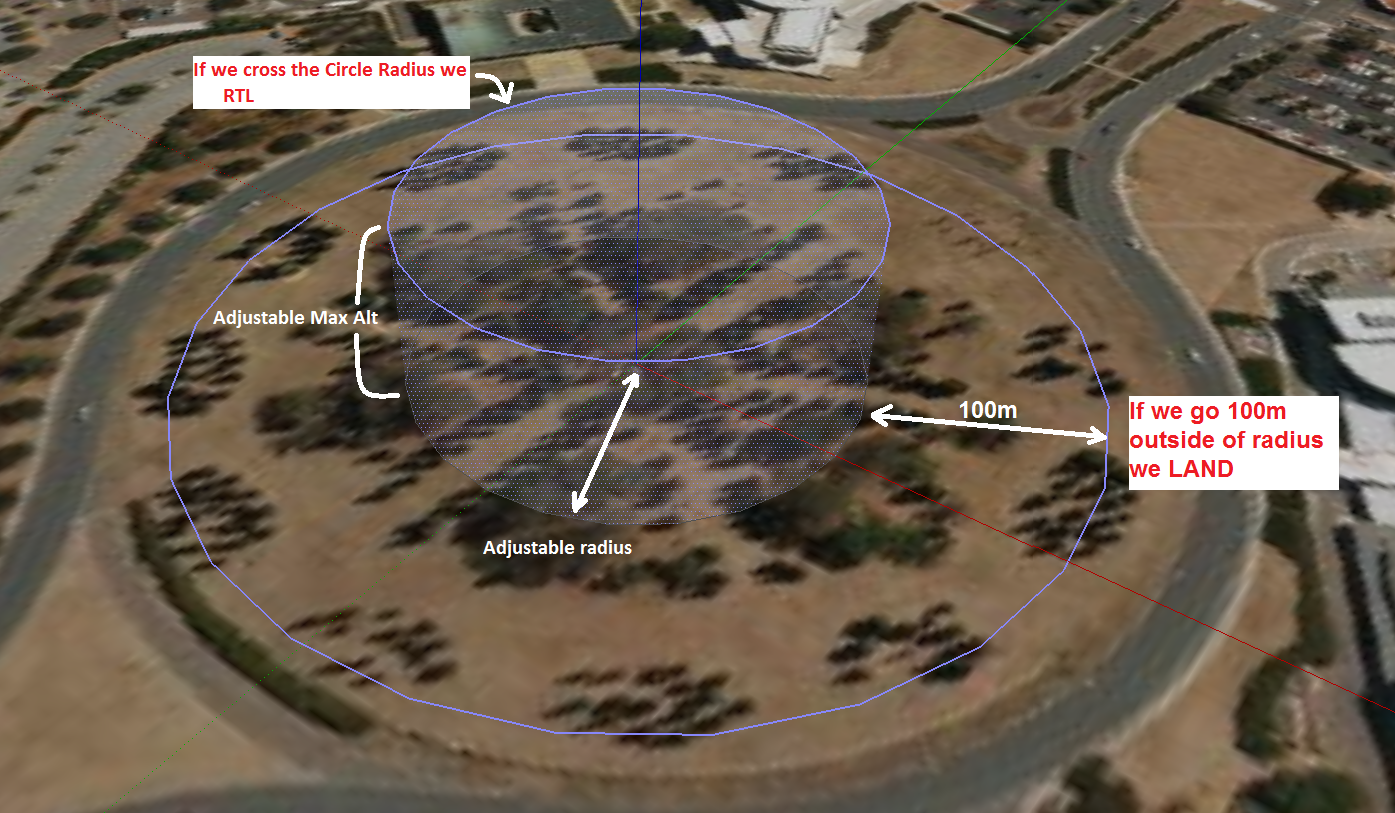
\includegraphics[scale=0.2]{images/apm_fence_1.png} 
\caption{Quelle: \url{http://copter.ardupilot.com/wp-content/uploads/sites/2/2012/12/Fence.png}}
\end{figure}
\end{frame}

\begin{frame}
\frametitle{Systembeispiel APM Planner/Mission Planner}
\begin{figure}
\begin{itemize}
\item Erlaubt live �berwachung mehrerer Dronen mittels GPS
\item Warnungen bei kritischen Ereignissen
\item GeoFence nimmt direkten Einfluss auf den Flug
\end{itemize}
\end{figure}

\end{frame}

\subsection{Use Cases}
%ableitung der use cases
\begin{frame}
\frametitle{Use Cases}
\begin{figure}
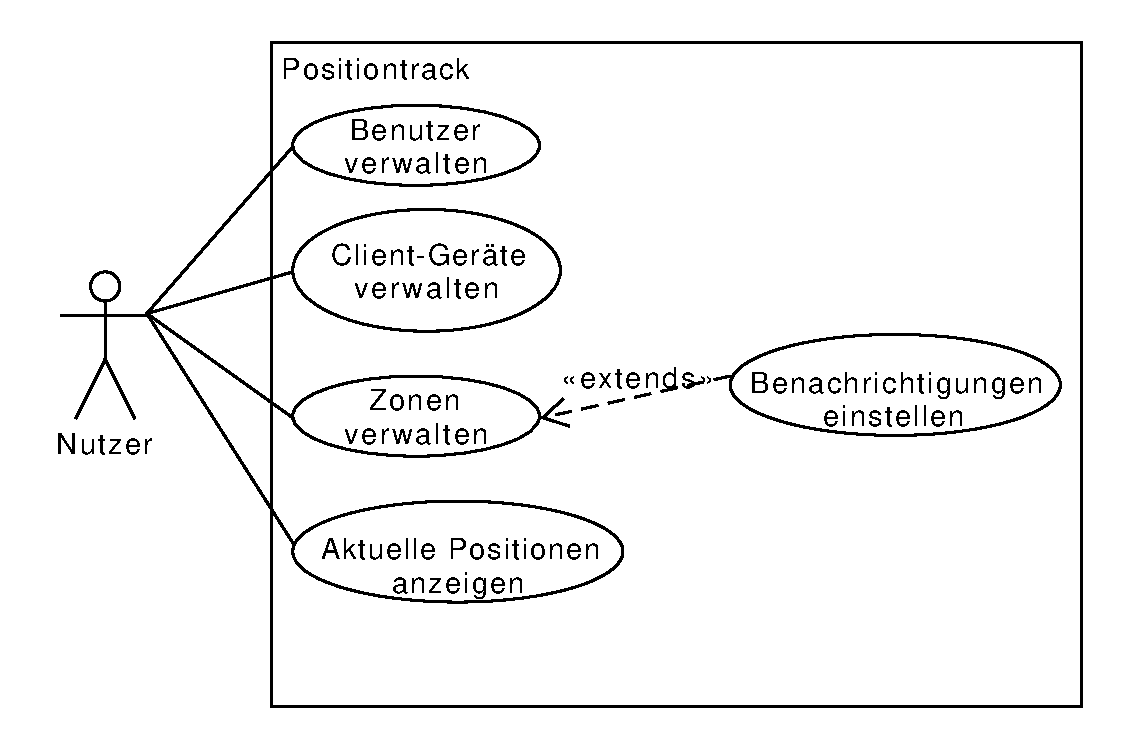
\includegraphics[scale=0.5]{images/useCaseDiagram.pdf}
\end{figure}
\end{frame}

\subsection{Systemanforderungen}
%aus allem vorher ableitung der systemanforderungen
\begin{frame}
\frametitle{Systemanforderungen}
\begin{itemize}
\item 
\item 
\item 
\item 
\item 
\item 
\end{itemize}
\end{frame}

%daraus architekturerstellung
\section{Architekturskizze}
%dazu gui mock
\begin{frame}
\frametitle{Architekturskizze}
\end{frame}

\begin{frame}
\frametitle{GUI Mock}
\begin{figure}
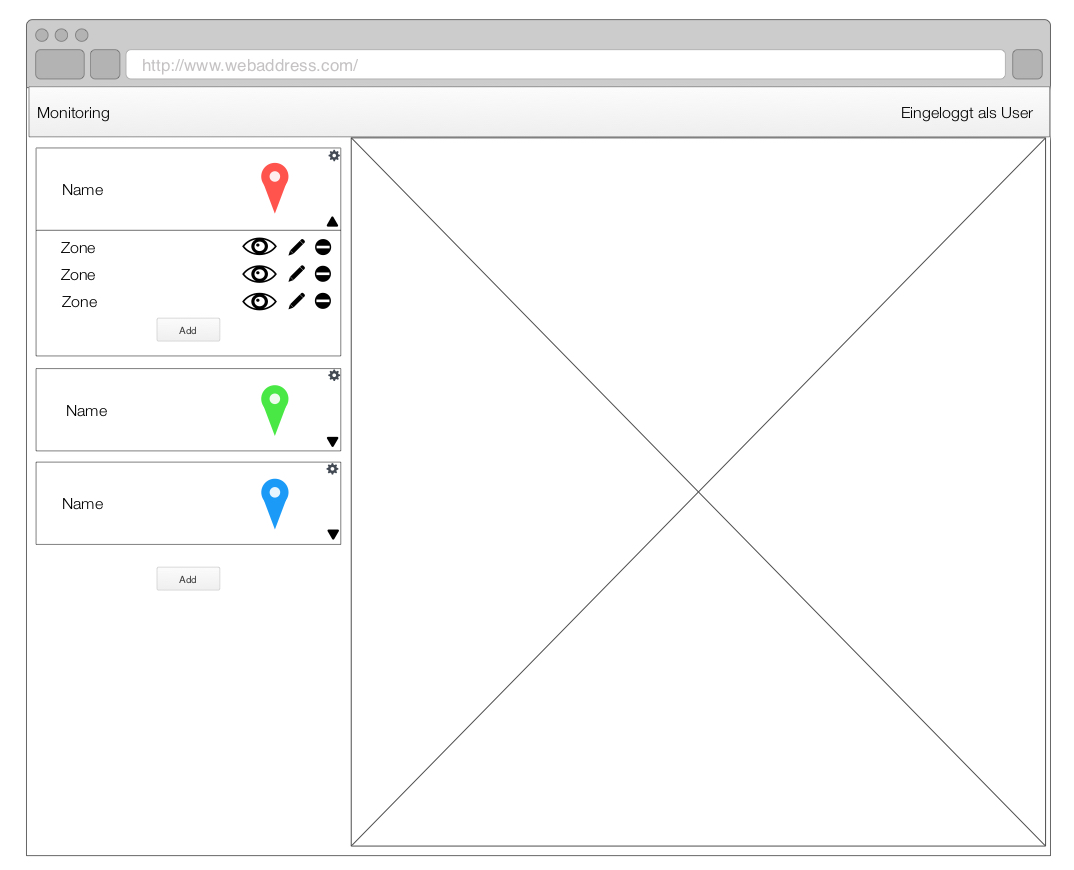
\includegraphics[scale=0.2]{images/gui_mock.jpg} 
\end{figure}
\end{frame}

%technologieentscheidungen
\section{Verwendete Technologien}
\begin{frame}
\frametitle{Verwendete Technologien}
\end{frame}



\section{Prototypvorstellung}
\begin{frame}
\frametitle{Prototypvorstellung}
\end{frame}

%was wird geleistet, was nicht? was w�ren die allerwichtigsten features/funktionen?
\section{Fazit}
\begin{frame}
\frametitle{Fazit}
\end{frame}

\beginbackup

\section*{Fragen?}

\begin{frame}
\begin{center}
\Huge{Fragen?}
\end{center}
\end{frame}

%\section{Literaturverzeichnis}

%\begin{frame}[plain, allowframebreaks]
%\frametitle{Literaturverzeichnis}
%\footnotesize
%\nocite{*}
%\beamertemplatetextbibitems
%\def\newblock{}
%\bibliographystyle{abbrvdin}
%\bibliography{literature}
%\end{frame}

\backupend

\end{document}